Jacobson~\cite{j1989} first proposed to design succinct data structures.
He showed how to represent an ordinal tree on $n$ nodes using $2n+o(n)$ bits so
that computing the first child, next sibling or parent of any given node
takes $O(\lg n)$ time in the bit probe model.
Clark and Munro~\cite{cm1996} showed how to support the same operations in
constant time in the word RAM model with word size $\Theta(\lg n)$.
Since then, much work has been done on succinct tree representations, to
support more operations, to achieve compression, to provide support
for updates, and so
on~\cite{mr1997,bdmr1999,grr2004,jss2007,ly2008,hms2012,fm2014,Navarro:2014:FFS:2620785.2601073}.
See Raman and Rao~\cite{rr2013} for a thorough survey.

Navarro and Sadakane~\cite{Navarro:2014:FFS:2620785.2601073} recently proposed a
succinct tree representation, referred to as NS-representation throughout this
paper, which was the first to achieve a redundancy of $O(n/\lg^c n)$ bits
for any positive constant $c$.
The \emph{redundancy} of a data structure is the additional space it uses above
the information-theoretic lower bound.
While all previous tree representations achieved a redundancy of $o(n)$ bits,
their redundancy was $\Omega(n \lg\lg n / \lg n)$ bits, that is, just slightly
sub-linear.
The NS-representation also supports a large number of
navigational operations in constant time (see
\cite{Navarro:2014:FFS:2620785.2601073} for details); only
the work in \cite{hms2012,fm2014} supports two additional operations.
An experimental study of succinct trees~\cite{ACNSalenex10} showed that
a simplified version of the NS-representation uses less space
than other existing representations in most cases and performs most operations
faster.
In this paper, we provide a parallel algorithm for constructing this
representation.

The NS-representation is based on the balanced parenthesis sequence $P$ of
the input tree $T$, which is obtained by performing a preorder traversal
of $T$ and writing down an opening parenthesis when visiting
a node for the first time and a closing parenthesis after visiting
all its descendants.
Thus, the length of $P$ is $2n$.

The NS-representation is not the first structure to use balanced parentheses to
represent trees.
Munro and Raman~\cite{mr1997} were the first to design succinct representations
of balanced parentheses and used them to represent ordinal trees succinctly by
reducing a set of navigational operations on trees to operations on their
balanced parenthesis sequences.
Their solution supports only a subset of the operations supported by the
NS-representation.
Additional operations can be supported using auxiliary data
structures~\cite{ly2008}, but supporting all operations supported by the
NS-representation requires many auxiliary structures, which add to the size
of the final data structure and make it complex in both theory and practice.
The main novelty of the NS-representation lies in its reduction of a large set
of operations on trees and balanced parenthesis sequences to a small set of
\emph{primitive operations}.
Representing $P$ as a bit vector storing a $1$ for each opening parenthesis
and a $0$ for each closing parenthesis, these primitive operations are the
following, where $g$ is an arbitrary function on $\{0,1\}$:
\begin{align*}
\sumop(P,g,i,j) &= \textstyle\sum_{k=i}^jg(P[k])\\
\fwdsearch(P,g,i,d) &= \min\{j \mid j \ge i, \sumop(P,g,i,j) = d\}\\
\bwdsearch(P,g,i,d) &= \max\{j \mid j \le i, \sumop(P,g,j,i) = d\}\\
\rmq(P,g,i,j) &= \min\{\sumop(P,g,i,k) \mid i\le k\le j\}\\
\RMQ(P,g,i,j) &= \max\{\sumop(P,g,i,k) \mid i\le k\le j\}\\
\rmqi(P,g,i,j) &= \argmin_{k\in[i,j]}\{\sumop(P,g,i,k)\}\\
\RMQi(P,g,i,j) &= \argmax_{k\in[i,j]}\{\sumop(P,g,i,k)\}
\end{align*}
Most operations supported by the NS-representation reduce to these primitives
by choosing $g$ to be one of the following three functions on $\{0,1\}$:
\begin{align*}
\pi : 1 &\mapsto 1 &\phi : 1 &\mapsto 1 & \psi : 1 &\mapsto 0\\
0 &\mapsto -1 & 0 &\mapsto 0 & 0 &\mapsto 1
\end{align*}
For example, assuming the $i$th parenthesis in $P$ is an opening parenthesis,
the matching closing parenthesis can be found using $\fwdsearch(P,\pi,i,0)$.
Thus, it (almost)\footnote{A few navigational operations cannot be expressed
  using these primitives.
  The NS-representation includes additional structures to support these
  operations.}
suffices to support the primitive operations above for
$g \in \{\pi, \phi, \psi\}$.
To do so, Navarro and Sadakane designed a simple data
structure called \emph{Range Min-Max Tree} ({\tt RMMT}).
It supports the primitive operations in logarithmic time when used to represent
the entire sequence~$P$.
To achieve constant-time operations, $P$ is further partitioned into chunks.
Each chunk is represented using an {\tt RMMT}, which supports primitive
operations inside the chunk in constant time if the chunk is small enough.
Additional data structures are used to support operations on the entire sequence
$P$ in constant time.

Next we briefly review the structure of the {\tt RMMT} and how it supports
the primitive operations for $g = \pi$.
Navarro and Sadakane~\cite{Navarro:2014:FFS:2620785.2601073} discuss how
to make it support these operations also for $\phi$ and $\psi$ while increasing
its size by only $O(n/\lg^c n)$.
To define the version of the {\tt RMMT} we implemented (and suggested by
Navarro/Sadakane as a simple practical structure), we partition $P$ into
disjoint chunks of size $s = w \lg n$, where $w$ is the machine word size.
For simplicity, we assume that the length of $P$ is a multiple of~$s$.
The {\tt RMMT} is a complete binary tree over the sequence of chunks
(see Figure~\ref{fig:RangeMinMaxTree}).
Each node $u$ of the {\tt RMMT} represents a subsequence $P_u$ of $P$ that is
the concatenation of the chunks corresponding to the descendant leaves of $u$.
Since the {\tt RMMT} is a complete tree, we do not need store to its structure
explicitly.
Instead, we index its nodes as in a binary heap and refer to each node by
its index.
The representation of the {\tt RMMT} consists of four arrays $e'$, $m'$,
$M'$, and $n'$, each of length equal to the number of nodes in the {\tt RMMT}.
The $u$th entry of each of these arrays stores some crucial information about
$P_u$:
Let the {\em excess} at position $i$ of $P$ be defined as $\sumop(P,\pi,0,i) =
\sum_{k=0}^{i} \pi(P[k])$.
$e'[u]$ stores the excess at the last position in $P_u$.
$m'[i]$ and $M'[i]$ store the minimum and maximum excess at any position in
$P_u$, respectively.
$n'[i]$ stores the number of positions in $P_u$ that have the minimum excess
value $m'[i]$.

\begin{figure}[t]
  \centering
  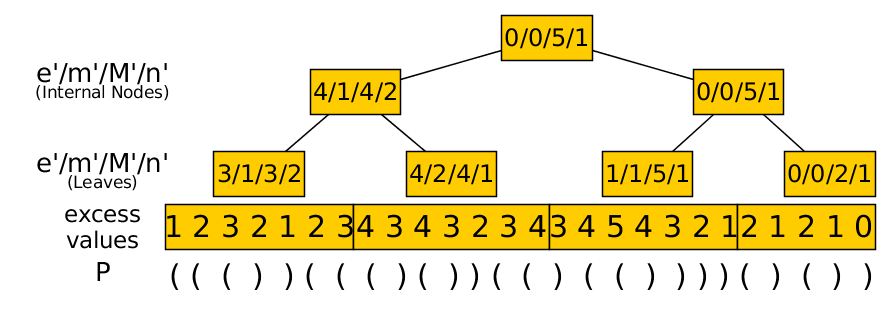
\includegraphics[scale=0.26]{./images/Range-min-max-tree.png}
  \caption{Range min-max tree}
  \label{fig:RangeMinMaxTree}
\end{figure}

Combined with a standard succinct data structure technique called {\em table
  lookup}, an {\tt RMMT} can support the primitive operations for $\pi$ in
$O(\lg n)$ time.
For example, consider $\fwdsearch(P,\pi,i,d)$.
We first check the chunk containing $P[i]$ to see if the answer is inside the
same chunk.
This can be done in $O(\lg n)$ time by breaking up the chunk into portions
of length $w/2$ and testing for each portion in turn whether it contains the
answer.
After constructing a universal lookup table whose content does not depend on
$P$, the test for each portion of length $w/2$ takes constant time: For each
possible bit vector of length $w/2$, and each of the $w/2$ position in the bit
vector, the table stores the answer of $\fwdsearch(P,\pi,i,d)$ if it can be
found inside this bit vector, or $-1$ otherwise.
As there are $2^{w/2}$ bit vectors of length $w/2$, this table uses
$2^{w/2}\poly(w)$ bits.
If we find the answer inside the chunk containing $P[i]$, the query terminates
and returns the answer.
Otherwise, let $u$ be the leaf corresponding to this chunk.
If $u$ has a right sibling, we inspect the sibling's $m'$ and $M'$ values to
determine whether it contains the answer.
If so, we let $v$ be this right sibling.
Otherwise, we move up the tree from $u$ until we find a right sibling $v$ of
an ancestor of $u$ whose corresponding subsequence $P_v$ contains the query
answer.
Then we use a similar procedure to descend down the tree starting from $v$ to
look for the leaf descendant of $v$ containing the result and spend another
$O(\lg n)$ time to determine the position of the query answer inside this leaf's
chunk.
Since we spend $O(\lg n)$ time for each of the two leaves inspected by this
procedure and the tests for any other node in the tree take constant time,
the cost is $O(\lg n)$.

Supporting operations on the leaves, such as finding the $i$th leaf from the
left, reduces to $\rankop$ and $\selop$ operations over another bit vector
$P_1[1..2n]$ where $P_1[i] = 1$ iff $P[i] = 1$ and $P[i+1] = 0$.
$\rankop$ and $\selop$ operations over $P_1$ in turn reduce to
$\sumop$ and $\fwdsearch$ operations over $P_1$ and can thus be supported
by an {\tt RMMT} for $P_1$.
$P_1$ does not need to be stored explicitly because any consecutive $O(w)$ bits
of $P_1$ can be computed from $P$ using table lookup.

To analyze the space usage, observe that storing $P$ requires $2n$ bits, while
the space needed to store the vectors $e'$, $m'$, $M'$, and $n'$ is
$2(n/s) \lg n = 2n/w$.
The space needed to store the same vectors for the {\tt RMMT} of $P_1$ is
the same.
Since we can assume that $w = \Omega(\lg n)$, the total size of the {\tt RMMT}
is thus $2n + O(n / \lg n)$.
